\documentclass[10pt, english, notes]{beamer}
\usepackage[normalem]{ulem}
\usepackage{graphicx}
\usepackage{ epstopdf}
\usepackage{enumerate}
\setbeamertemplate{itemize item}[square]
\setbeamertemplate{itemize subitem}[triangle]
\setbeamertemplate{itemize subsubitem}[circle]
\setbeamertemplate{navigation symbols}{}
%\addtobeamertemplate{navigation symbols}{\small{\insertframenumber/\inserttotalframenumber}}
\usepackage{mathptmx}
\usepackage[T1]{fontenc}
\usepackage[utf8]{inputenc}
\usepackage{color}
\usepackage{fancybox}
\usepackage{calc}
\usepackage{ifsym}
\usepackage{amsmath}
\usepackage{amssymb}
\usepackage{babel}
\usepackage[autoplay, palindrome]{animate}
\usepackage{lastpage}
% \usepackage{multimedia}
\usepackage{movie15}
% \usepackage[pdftex]{graphicx}
\usepackage{epstopdf}
\mode<presentation>
{
  \usetheme{Warsaw}
  % \useoutertheme{infolines}
  \useoutertheme{shadow}
  \usecolortheme{beaver}
  % \usefonttheme{serif}
  % \usecolortheme{wolverine}
  % \usecolortheme{whale}
  \setbeamercovered{transparent}
}
% -----------------------------------------------------------------------
% Configuration de l'environnement Nota
\RequirePackage{Styles/Nota}
\newcommand{\ficnota}{Styles/Attention}
\newcommand{\ficnote}{Note}
\newcommand{\ficnotahack}{Question}

\setlength{\largeurnota}{.8cm}
\newenvironment{Nota}{%
  \begin{pictonote}{\ficnota}}{\end{pictonote}}
\newenvironment{Note}{%
  \begin{pictonote}{\ficnote}}{\end{pictonote}}
\newenvironment{Notahack}{%nn
  \begin{pictonote}{\ficnotahack}}{\end{pictonote}}
% -----------------------------------------------------------------------
% \usepackage{palatino}
\title[Training: GUI]{Training: Graphical User Interface\footnote{Visit: \url{http://www.mathworks.com/help/matlab/ref/guide.html}}
	(\raisebox{0pt}  {\rotatebox{10}{G}}
     	\raisebox{-2pt}  {\rotatebox{-10}{U}}
     	\raisebox{0pt}    {\rotatebox{10}{I}})
\\}
%[~~~~~~~~~~~~~~\thepage/\pageref{LastPage}] 
\author[A. MHAMDI] {Abdelbacet MHAMDI
\bigskip{}
\\{\href{mailto:Abdelbacet.MHAMDI@gmail.com}{\textifsymbol{0} \textcolor{blue}{Abdelbacet.MHAMDI@gmail.com}}}
\bigskip{}
\\ Automatic Control and System Design Engineering}
\institute[ISET de Bizerte]{Institut Supérieur des \'Etudes Technologiques de Bizerte}
\date[] {\textsc{(** *** 2014)}}
\subject{Getting Started with GUI}
\AtBeginSection[]
% \AtBeginSubsection[]
{
 \begin{frame}<beamer>{Outlines}
  \tableofcontents[currentsection, currentsubsection]
  \end{frame}
}
%%%%%
\hypersetup{
% pdfpagemode = FullScreen, % afficher le pdf en plein ecran
pdfauthor = {A. MHAMDI}, %
pdftitle = {GUITraining}, %
pdfsubject = {Getting Started with GUI}, %
pdfkeywords = {Labs, GUI, Engineer},%
% pdfcreator = {PDFLaTeX}, %
% pdfproducer = {PDFLaTeX} %
}
%%%%%
% \logo{\includegraphics[height=5mm]{SimLogo.png}}
\begin{document}
\begin{frame}[plain]{}
% 
\includegraphics[scale = 0.25, angle = 0]{IsetLogo}
\titlepage
\end{frame}
%%%%%
\begin{frame}{Preface}
\thispagestyle{empty}
\begin{Nota}
The Url shown in footnotes are indicatives. They have been visited in $2014$. We do not guarantee their validities and we are not responsible on updates mis-leaded by some websites.
\end{Nota}
\pause
\begin{block}{Purposes}
	\begin{itemize}
		\item <alert@2>Create a Graphical User Interface to acquire video streaming.
		\item <alert@3>Deploy the project to get an application running on windows machine.
	\end{itemize}
\end{block}
% \begin{center}
% 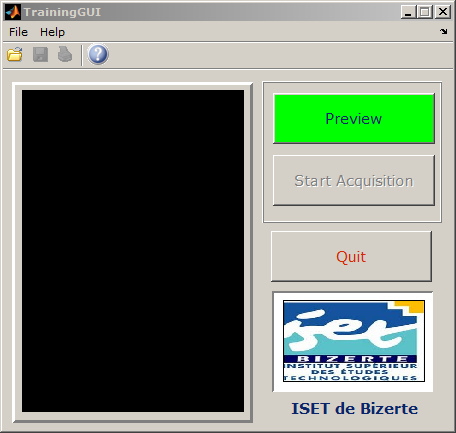
\includegraphics[height = 4cm, width = 6.5cm]{GUI/GUInterface}
% \end{center}
\end{frame}
%%%%%
\begin{frame}{Outlines}
\tableofcontents
\end{frame}
%%%%%
\section{Honor Code}
\begin{frame}{Taken from another university}
\framesubtitle{(THE UNIVERSITY of NORTH CAROLINA at CHAPEL HILL: Department of Physics and Astronomy\footnote{See: \url{http://physics.unc.edu/undergraduate-program/labs/general-info/}})}
During this course, you will be working with one or more partners with whom you may discuss any points concerning laboratory work. However, you must write your lab report, in your own words. 
\par
Lab reports that contain identical language are not acceptable, so do not copy your lab partner's writing.
\par
If there is a problem with your data, include an explanation in your report. Recognition of a mistake and a well-reasoned explanation is more important than having high-quality data, and will be rewarded accordingly by your instructor. A lab report containing data that is inconsistent with the original data sheet will be considered a violation of the Honor Code.
\end{frame}
%%%%%
\begin{frame}
Falsification of data or plagiarism of a report will result in prosecution of the offender(s) under the University Honor Code.
\par
On your first lab report you must write out the entire honor pledge:
\par
\setbeamercolor{block body alerted}{fg=white, bg=red}
\begin{alertblock}{}
\centering
"The work presented in this report is my own, and the data was obtained by my lab partner and me during the lab period."
\end{alertblock}
\par
On future reports, you may simply write \emph{"Laboratory Honor Pledge"} and sign your name.
\end{frame}
%%%%%
\section{What is a GUI?}
\begin{frame}{}
\begin{alertblock}{Definition\footnote{What Is a GUI? - MATLAB \& Simulink \url{http://www.mathworks.com/help/matlab/creating_guis/what-is-a-gui.html}}}
\begin{itemize}
\item A \uline{G}raphical \uline{U}ser \uline{I}nterface (\textit{GUI}) is a graphical display containing components that enable a user to perform interactive tasks.
\item GUI components can include menus, toolbars, push buttons, radio buttons, list boxes, and sliders, etc. 
\item GUIs created using MATLAB® tools can also perform any type of computation, read and write data files, communicate with other GUIs, and display data as tables or as plots.
\end{itemize}
\end{alertblock}
\textcolor{blue}{Click \href{http://www.youtube.com/user/eeprogrammer}{\beamergotobutton{here}} to subscribe on YouTube for further tutorials.}
\begin{block}{Hierarchy}
\begin{center}
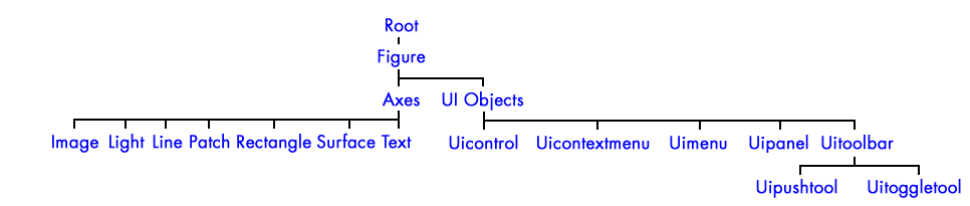
\includegraphics[scale = 0.4, angle = 0]{GUI/Hierarchie}
\end{center}
\end{block}
\end{frame}
%%%%%%%%%%%%%%%%%%%%%%%%%%%%%%
\begin{frame}{GUI Sketch}
\begin{center}
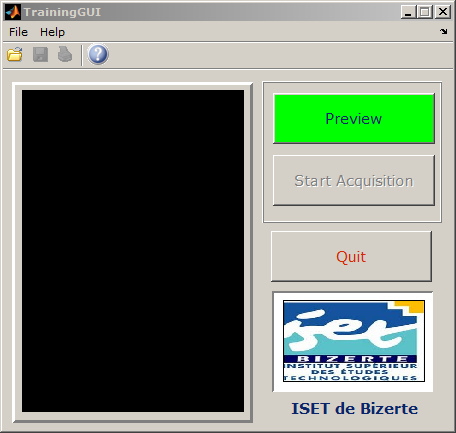
\includegraphics[height = 7cm, width = 11cm]{GUI/GUInterface}
\end{center}
\end{frame}
%%%%%%%%%%%%%%%%%%%%%%%%%%%%%%
\begin{frame}{Lab. \footnotesize{(Matlab R2011a)}}
\begin{center}
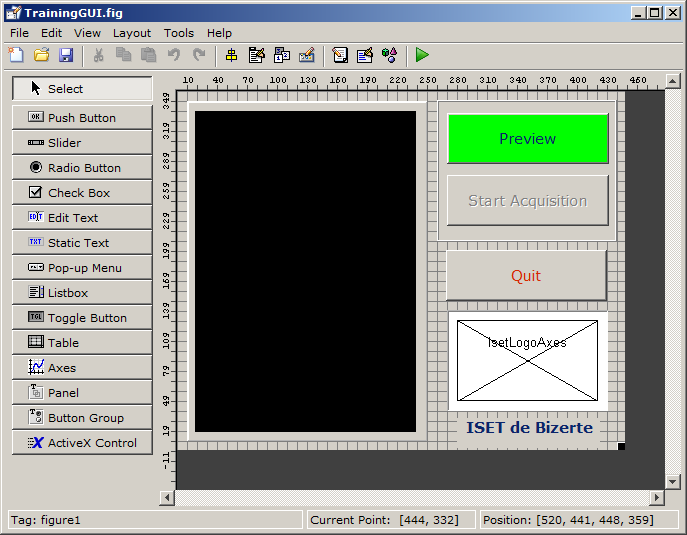
\includegraphics[height = 7cm, width = 11cm]{GUI/GUIGuide}
\end{center}
\end{frame}
%%%%%%%%%%%%%%%%%%%%%%%%%%%%%%
\section{Deploy Tool}
\begin{frame}{Overview}
MATLAB Compiler™ lets you share MATLAB® programs as standalone applications or shared libraries for integration with common programming languages\footnote{\url{http://www.mathworks.com/products/compiler/}}.
\begin{center}
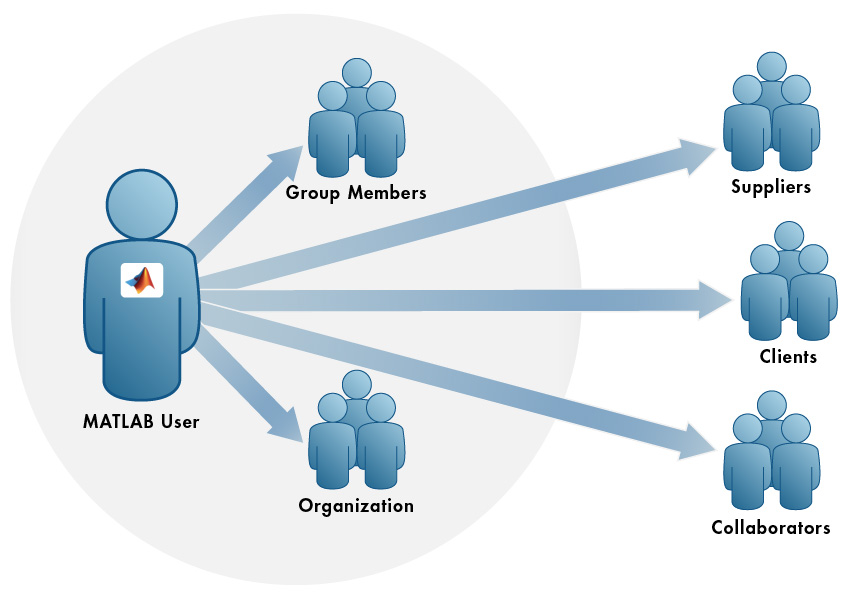
\includegraphics[scale = 0.25, angle = 0]{GUI/MatLabSharing}
\end{center}
\end{frame}
%%%%%%%%%%%%%%%%%%%%%%%%%%%%%%
\begin{frame}{Compiler Specification}
\begin{center}
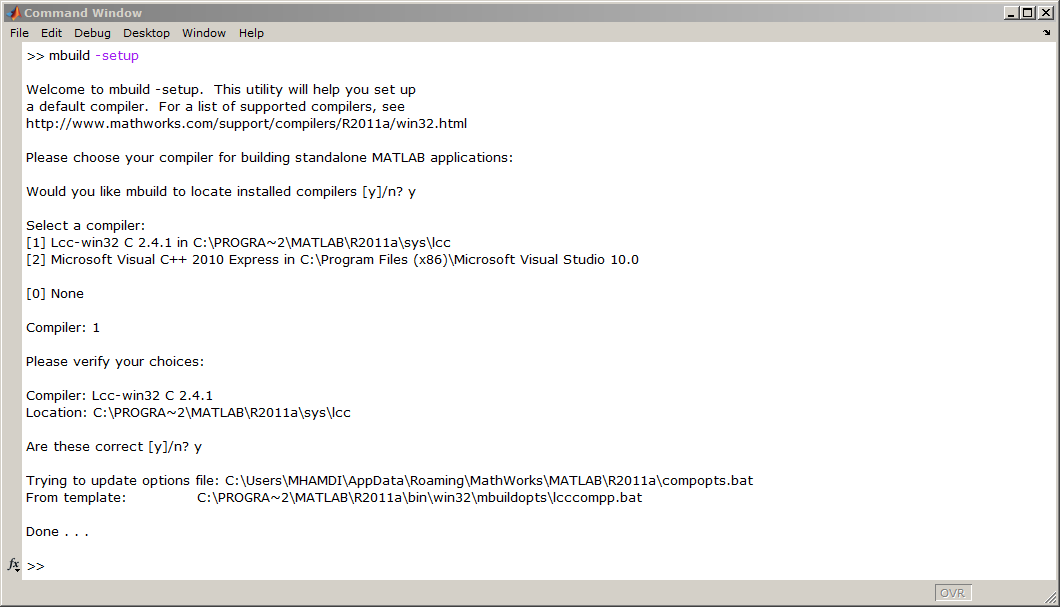
\includegraphics[height = 7cm, width = 10cm]{GUI/LCCCompiler}
\end{center}
\end{frame}
%%%%%%%%%%%%%%%%%%%%%%%%%%%%%%
\begin{frame}{Architecture of Compilation under MATLAB}
Applications and libraries created with MATLAB Compiler use the MATLAB Compiler Runtime, which enables royalty-free deployment to users who do not have MATLAB\footnote{\url{http://www.mathworks.com/products/compiler/}}.
\begin{center}
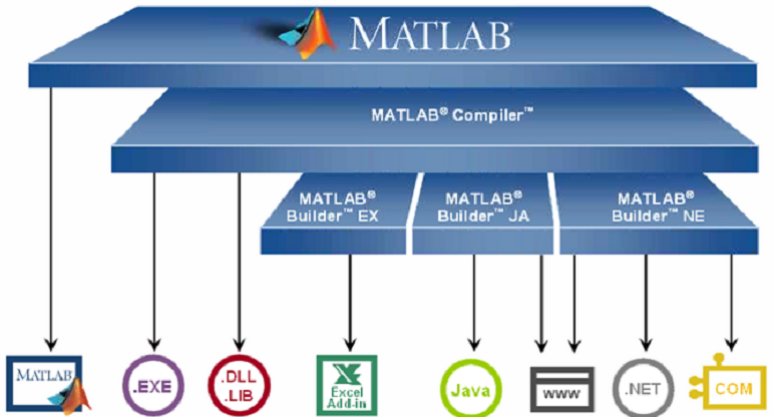
\includegraphics[scale = 0.4, angle = 0]{GUI/DeployPic}
\end{center}
\end{frame}
%%%%%%%%%%%%%%%%%%%%%%%%%%%%%%
\begin{frame}{Procedure (1/2)}
\begin{columns}
\begin{column}{5cm}
\begin{figure}
\centering
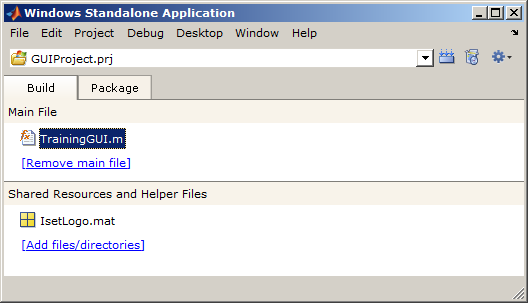
\includegraphics[height = 5cm, width = 5cm]{GUI/DeployPro}
\caption{Adding files}
\end{figure}
\end{column}
\begin{column}{5cm}
\begin{figure}
\centering
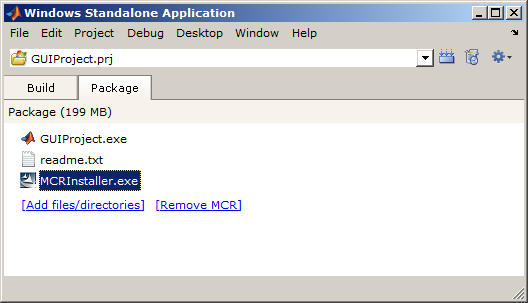
\includegraphics[height = 5cm, width = 5cm]{GUI/DeployProConf}
\caption{Packaging of Matlab Component Runtime (MCR)}
\end{figure}
\end{column}
\end{columns}
\end{frame}
%%%%%%%%%%%%%%%%%%%%%%%%%%%%%%
\begin{frame}[fragile]{Procedure (2/2)\footnote{\url{http://www.mathworks.com/matlabcentral/answers/101376-how-do-i-associate-a-custom-icon-with-an-exe-compiled-with-the-matlab-compiler-4-0-r14}}}
\setbeamercolor{block body alerted}{fg=red, bg=yellow}
\begin{alertblock}{}
\centering
This is not possible in releases R2010b-R2013a.
\end{alertblock}
\begin{enumerate}
\item Choose an icon 
\includegraphics[scale = 0.4, angle = 0]{GUI/MyIcon}. Rename it as \emph{"MyIcon.ico"}.
\item Create a new text file and write \alert{"ConApp ICON \emph{MyIcon.ico}"} in it. Rename it as \emph{"MyIconResource.rc"} and save it in your current directory.
\item Compile \emph{"MyIconResource.rc"} and \emph{"MyIcon.ico"} files using the following command at MATLAB prompt:
\begin{verbatim}
system(['"' matlabroot '\sys\lcc\bin\lrc" /i "' ...
                          ...pwd '\MyIconResource.rc"']);
\end{verbatim}
\item Compile the MATLAB files and the resource file together using the -M option as before:
\begin{verbatim}
mcc -m TrainingGUI.m -M myiconresource.res -o My GUI -v
\end{verbatim}
\end{enumerate}
\end{frame}
%%%%%%%%%%%%%%%%%%%%%%%%%%%%%%
\begin{frame}{The End.}
\thispagestyle{empty}
\begin{center}
\textcolor{blue}{\Huge Thanks a lot for attending~}
\par
\textcolor{blue}{\Huge this training.}
\end{center}
\end{frame}
%%%%%
% \begin{frame}[plain]{}
% \includegraphics[scale = 0.25, angle = 0]{EspritLogo}
% \titlepage
% \end{frame}
%%%%%%
\end{document}

